\subsection{Literature review}

\quad After the post-pandemic recovery phase inflation rose from disturbances on the supply side, first with supply-chain disruptions and then with the energy crisis from the war in Ukraine, GDP growth has slowed to a standstill, and business confidence remained below its long-term average. 
Yet, the different labour markets across Europe are not showing strong signs of weakening, and record low unemployment levels conversely point to highly tight markets. 
If inflationary pressures were to strongly pass-through to wages, once the energy crisis and induced effects (rising prices for commodities, food, transportation costs\dots) fade, wage growth could play a key role in inflation not returning to normal levels, especially if the pass-through is slow. 
We could see inflation going down before rising due to increasing consumer spending power through delayed wage increases. Thus, the keen interest in inflation and the interaction with wages being a key challenge for monetary policy motivated our study of wage dynamics, especially regarding the Eurozone labour market outlook for this publication. 

The primary basis for our study was to extend a Goldman Sachs study on the drivers of wage growth in the UK to the Eurozone Big 4, namely France, Germany, Spain, and Italy. 
Through a large range of model specifications, they assessed the extent to which the labour market needs to cool down to bring down wage growth and thus possibly inflation.
From the estimated Phillips curve the drivers of recent wage growth strength are derived, highlighting a strong effect of a tight labor market and high inflation expectations mix.
Coefficients estimates also allow the authors to evaluate what it would take to bring down wage inflation to levels usually considered compatible with the BoE inflation target.

Phillips curve models have longed been studied from the original 1958 paper \textit{"The Relation between Unemployment and the Rate of Change of Money Wage Rates in the United Kingdom, 1861-1957"}\cite{labour0} to most recent studies on its possible weakening explainability power due to flattening during the pandemic (Hartwig, Nickel \& Bobeica (2021)\cite{labour1}). 
In their 2017 chapter of the IMF World Outlook on drivers of wage growth Nabar \& al.\cite{labour2} consider the Phillips curve framework proposed by Gali in 2011\cite{labour3} and illustrate the expected weights of inflation expectations and productivity growth on wage growth. 
While in the original paper from Williams Phillips the link is drawn between nominal wage growth and unemployment in Great Britain, it appears from their results that despite slack being a known key driver of wage development, the unemployment rate alone may not adequately capture all constraints in the labor market leading to wage inflation, and thus other measures of slack should be considered.

This is consistent with a broader literature as measures regarding slack have largely been discussed. 
Recently, Domash \& H. Summers (2022)\cite{labour4} from the Centre for Economic Policy Research (CEPR) provided an in-depth analysis of a wide range of alternative measures of slack in the US, particularly measures that include a demand dimension, to assess labor market tightness. 
They also highlighted the changes, amid the pandemic, in these measures that used to move together but started behaving differently. 
This induces a growing interest to consider them separately and not as interchangeable measures. 
Moreover, they point out the instability of estimated relationships between wage developments and the slack measures -whether it is due to stationary properties of some variables or structural changes- and raise caution when one attempts to predict future wage growth. 
Both Saez \& Michaillat (2022)\cite{labour5} and Furman \& Powell (2021)\cite{labour6} also illustrated the better fit of job vacancy rate and quit rate as demand-side slack measures in the US.

In the ECB Economic Bulletin of January 2023, Bodnár \& al.\cite{labour7} shed light on measures’ differences but this time regarding wage growth as the latter also started showing some divergence during the pandemic. 
Namely, the annual growth of compensation per employee (consisting of total wages and salaries paid by employers but also of imputed social contributions, expressed per employee) decreased while the compensation per hour and the Labor cost index from Eurostat both rose during the same period. 
Despite moderating over time some differences still remain. 
As the goal of our analysis is not to highlight these differences we chose not to focus on this issue but it is still worth mentioning. 
We give more precision regarding the selection of our variables in the dedicated data section.

More recently, and in line with our study, Domash \& H. Summers (2023)\cite{labour8} assessed the recent wage development in the US and argue that the traditional Phillips Curve framework still performs relatively well when predicting wage inflation. 
Moreover, they underline the factors that would bring down wage growth to levels compatible with the Federal Reserve’s 2\% inflation target.

We build on this literature and make the following main contributions: investigating broader slack measures for European countries and estimating Phillips curves with a rich dynamic structure following our own methodology. 
Our model sheds light, both quantitatively and qualitatively, on the relative importance of the key wage drivers, all the more highlighted over time by the contribution breakdown charts, while performing fairly well. 
We are thus able to strengthen the Eurozone Labour market outlook for Allianz Trade’s quarterly outlook. 
In hindsight even though we were satisfied with the results we also point out limits and overall reflections we have on the methodology throughout the report.
\subsection{Data and Methodology}
\subsubsection{Data}

\quad \textbf{Wage.} As our study did not focus on the different possible measures of wage and the inherent differences mentioned in particular by Bodnár \& al.\cite{labour7} we decided to construct a simple measure that would be comparable across countries. 
Our wage variable $Wage$ is more of a labour cost variable than a, strictly speaking, wage measure. We take the logarithm of the Hourly earn in 2015 basis (2015=100). 

\textbf{Inflation.} The standard Phillips curve relies on an inflation expectation variable. 
However, as we not only aimed to study the drivers of inflation through the Phillips curve framework but also to produce some forecasts and a forward-looking assessment of the different labour markets we decided to switch the inflation expectation variable to realised inflation. 
With the team making inflation forecast scenarios every quarter we are then confident in the data and we do not rely on some external source for this specific variable. 
It also makes it really easy to consider different inflation pathways if need be. 
Thus, our inflation variable $CPI$ is simply measured by the logarithm of the Consumer Price Index (2015=100) of all items.

\textbf{Productivity.} We measure labour productivity, or just productivity, as the logarithm of the four-quarter moving average of the Gross Domestic Product (produced at each quarter) to employment ratio. 
We take a moving average rather than the direct ratio for two reasons: to smoothen the overall curve and remove possible base effects and as productivity changes may not instantly translate into wages, but rather productivity trend changes affect wage growth, we decided that the trend of productivity growth would be deemed more appropriate.

\textbf{Labour underutilisation.} As discussed in the introduction we consider several different slack measures. 
Our first variable of labour underutil is the Unemployment ($U$) measured the country-specific unemployment rate. 
We then also considered the following measures: the Job-Worker Gap as a share of the labour force ($JW\textrm{-}LF$) measured by the ratio between the job-worker gap (labour demand [employment + job vacancies/openings] minus labour supply [employment + unemployment]) and the labour supply in percentage; the Vacancies to Unemployment ratio ($V/U$) and the Labour force Participation rate ($LF\textrm{-}part$) measured by the logarithm of the ratio between the Labour supply and the Population in working age.
Some variables remained missing for some countries though, see Figure \ref{figure:Labour_ur}.

We start by running some unit root tests on our variables to assess their level of stationarity.
Find below a result table summarising the key results from the different tests.

\begin{figure}[H]
    \centering
    \caption{\textit{Unit root test results by country and variable, in level and first difference.}}
    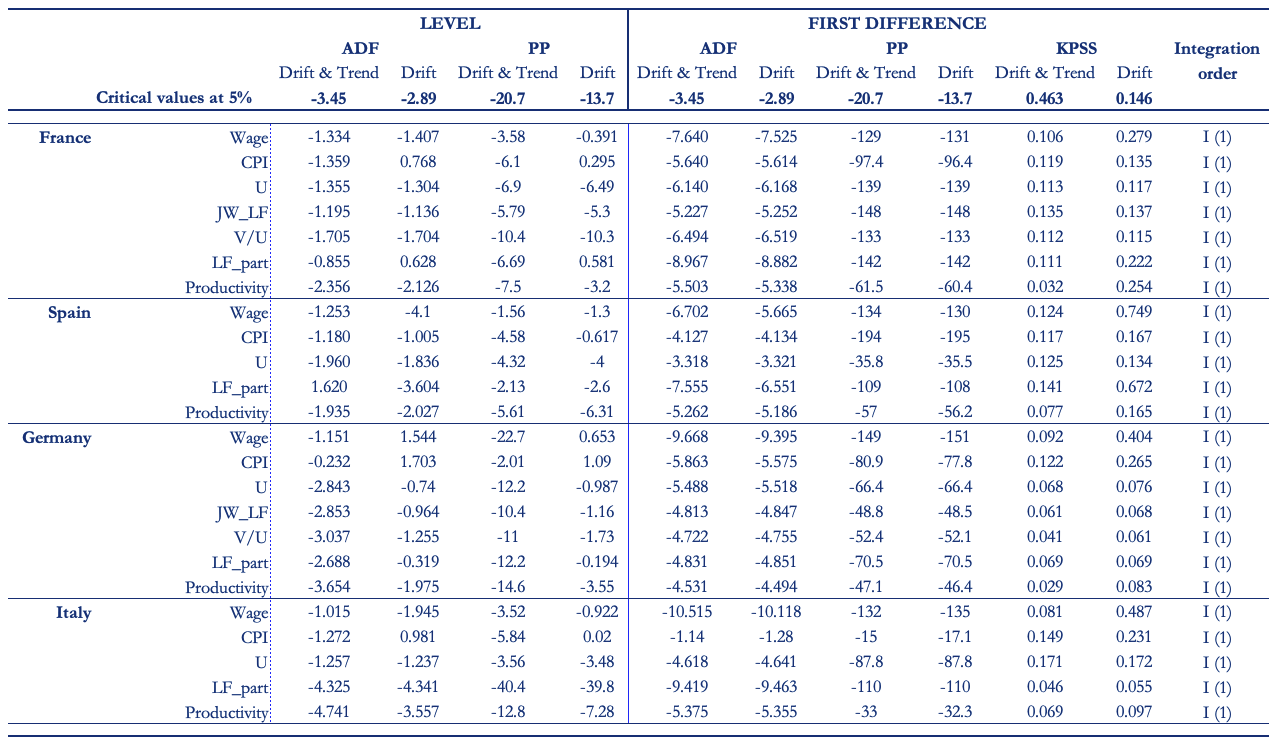
\includegraphics[width=1\textwidth]{Core/2.Labour/img/unit_root.png}
    \label{figure:Labour_ur}
\end{figure}
\vspace{-1cm}
We use the standard Augmented Dickey-Fuller (ADF) and Perron-Phillips (PP) tests to asses the different series showing signs of a unit root in level. 
As a reminder the null hypothesis for both the ADF and PP test is the presence of a unitary root and thus non-stationary. 
We run the ADF test with Drift (\ref{adf1}) \& Trend and with Drift only (\ref{adf2}). Likewise for the other tests. To check that the stationary hypothsis is not incorrect for the first difference series we use the KPSS test, where the null hypothesis is stationarity.
\begin{align}
    \Delta y_{t} = \gamma y_{t-1} + a_{0} + a_{1}t + \sum_{i=2}^{p}\beta_{i} \Delta y_{t-i+1} + \epsilon_{t} \quad \longmapsto \; \textrm{H(0): } \gamma = 0 \label{adf1} \\
    \Delta y_{t} = \gamma y_{t-1} + a_{0} + \sum_{i=2}^{p}\beta_{i} \Delta y_{t-i+1} + \epsilon_{t} \quad \longmapsto \; \textrm{H(0): } \gamma = 0 \label{adf2}
\end{align}
\quad After computing the first difference counterpart for each series we interpret the comparison of either the Drift \& Trend or Drift statistics to its corresponding critical value depending on the differentiated series looks. 
Overall all series are not level-stationary as the  t-statistics for the ADF and PP are below the critical values, we thus can’t reject the presence of a unit root. 
Running the same test on the differentiated series establishes the series as first-difference-stationary. Using the KPSS test the hypothesis of stationarity cannot be rejected at the 5\% level, thus reinforcing our conclusion of the variables being integrated of order one I(1).

\subsubsection{Methodology and Model selection}
\quad As we highlighted in the previous section, our variables are I(1) and we thus consider a model ran in first difference. Namely, we run country-specific Autoregressive Distributed Lag (ARDL) models of the following form:
\begin{equation*}
    \Delta wage_{t} = \sum_{k=1}^{W}\alpha_k \Delta wage_{t-k} + \sum_{k=0}^{Q}\beta_k^{(CPI)} \Delta CPI_{t-k} + \sum_{k=0}^{S}\beta_k^{(slack)} \Delta slack_{t-k} + \sum_{k=0}^{P}\beta_k^{(prod)} \Delta prod._{t-k} + \theta_{1}\mathbb{1}_{covid} + \theta_{2}\mathbb{1}_{GFC}
\end{equation*}
For $t=1,\ldots,T$ and where the maximum lags $\left\{Q,S,P\right\}\in\left[0;6\right]\ and\ \left\{W\right\}\in\left[1;6\right]$ ($prod.$ refers to the Productivity variable).

The model is estimated via Conditional Maximum Likelihood (\textit{using the ARDL framework from the statsmodel python package}) on a quarterly basis from Q2 1997 to Q4 2022 for Germany, France and Spain. 
For Italy, the sample only starts in Q1 1998. As our goal is to assess recent wage developments and produce monitoring models for our outlook it is mandatory we include as much data as possible. 
Thus, $\mathbb{I}_{covid}$ is a dummy variable over the Covid-19 period (2020Q1 – 2022Q2) included to alleviate to a certain extent the disruption in the data associated with the crisis but external to the explanatory variables included. 
There is also a dummy variable for the Global Financial Crisis (2007Q2 – 2009Q1). 
Since the economic theory does not provide guidance regarding the number of lags to include we decided to restrict the equation to include lags up to 6 quarters, i.e up to a year and a half, as we assumed there could be some links with the previous year for some variables but going up to 8 quarters might go overboard and introduce too much variance.

For the wage ($Wage$), inflation ($CPI$) and labour productivity ($prod.$) variables the interpretation of the first difference series is straightforward as it produces quarter-on-quarter growth rates (\%QoQ) of the said series. 
Then, we have several country-specific equations depending on the slack measure chosen (slack). 
As for the latter, the interpretation of the first difference varies across measures but it is either a QoQ growth rate for the labour force participation ($LF\textrm{-}part$) or QoQ differences for the other three ($U$, $JW\textrm{-}LF$, $V/U$). 
The model includes both some autoregressive momentum, with the lag wage components, and the dynamic of predictor variables. 
The rationale behind the inclusion of more than one lag compared to the theoretical framework and a simple regression model is more or less the following. 
Firstly, a richer structure could perform better in a purely statistical perspective and would thus allow building up a better outlook with stronger confidence. 
But as we track multiple countries the maximum lag selection could also corroborate or at least provide further information on particular features of individual context. It could be the dragging or quick adjustment of wage growth changes across time, the extent of inflation pass-through to wages (especially if only recent quarters in inflation changes matter or if the changes from the past year still carry heavy weights), with the latter being a central issue in policy discussion when it comes to tackling high inflation and taking into account the labour market situation. 
These are some of the many questions that we attempt to address using our model framework complementary to assessing the differences in the choice of slack measures.

Thus, with the two-fold objective of investigating broader slack measures and producing country-specific labour market outlooks, our model selection is composed of multiple steps. 
First, we run all possible model combinations of maximum lags included for each variable. 
Then, as we investigate this broad range of models we are able to select the \textit{‘best’} ones from a statistical perspective (one per slack measure variable) with the minimisation of the Akaike Information Criterion (AIC). 
Moreover, the pool of models is beforehand reduced as we only consider structures, where every maximum lag included, is significant at the 10\% level. 
This first step combines the classical tools which are information criterion and statistical tests.

However statistically good the models described above might be, the selection of one as the best still lacks some economic fundamentals. 
More than just including lags of explanatory variables, the ARDL framework provides a feature that we tried to leverage to a certain extent to control our pool of possible models and make sense of their statistical features in an economic sense. 
Using the regression equation we can compute the dynamic marginal effect of each variable lag included, known as short-run effects $\frac{\mathrm{d}y_{t}}{\mathrm{d}x_{t_{i}}}$. 
If we consider a permanent unitary shock in $X_{t}$ so that $E(X_{t})$ changes, the effect in $E(Y_{t})$ is (\ref{eq1}), known as the long-run multiplier (LRM). The latter is also the accumulation of short-run effects. 
With stationary series and white noise $\epsilon_{t}$ we have, using $\theta (L) = 1 - \theta_{1}L - \theta_{2}L^{2} - \dots - \theta_{p}L^{p}$ and $\phi (L) = \phi_{0} + \phi_{1}L + \phi_{2}L^{2} + \dots + \phi_{q}L^{q}$:
\vspace{-0.3cm}
\begin{align}
    \theta (L)y_{t} &= \delta + \phi (L)x_{t} + \epsilon_{t} \nonumber \\
    y_{t} &= \theta^{-1} (L)\delta + \theta^{-1} (L)\phi (L)x_{t} + \theta^{-1} (L)\epsilon_{t} \nonumber \\
    \frac{\mathrm{d}E(y_{t})}{\mathrm{d}E(x_{t})} &= \theta^{-1} (L)\phi (L).1 = \theta^{-1} (1)\phi (1) \nonumber\\
    \frac{\mathrm{d}E(y_{t})}{\mathrm{d}E(x_{t})} &= \frac{\phi_{0} + \phi_{1} + \phi_{2} + \dots + \phi_{q}}{1 - \theta_{1} - \theta_{2} - \dots - \theta_{p}} \label{eq1}
\end{align}

We utilise this long-run multiplier as a constraint in our model selection process.
We argue that a one per cent permanent increase in $\Delta CPI$ and $\Delta prod.$ variables, namely a one per cent permanent increase in QoQ inflation and productivity growth should be associated with a positive long-run multiplier for wage growth. 
We thus add another step in our model selection with an expected sign constraint on the LRM for each computed model. 
On the other hand for the different slack measures, we do not impose any constraint on the LRM sign. 
Through the Okun law, which links changes in unemployment and GDP growth, we argue that it is best to let LRM associated with the chosen slack measure unconstrained, despite the expectation we could have on its sign.
\vspace{-0.0005cm}
\begin{align*}
    \frac{\Delta Y}{Y} = k - c\Delta U \underset{\textrm{unitary shock on U}}{\longrightarrow} \hspace*{0.7cm} \frac{\Delta Y}{Y} &= k - c(\Delta U + 1)\\
    \frac{\Delta Y}{Y} &\geqslant 0 \Leftrightarrow k - c\Delta U \geqslant c\\
    \frac{\Delta Y}{Y} &\geqslant 0 \Leftrightarrow \frac{k}{c} \geqslant \Delta U +1\\
\end{align*}
\quad Thus, the last line shows that the effect of a unitary shock to $\Delta U$ on GDP growth is not straightforwardly clear, as it depends on the state of $\Delta U$ compared to the constant $\frac{k}{c} - 1$. 
If we are in a situation where the effect of a shock on the unemployment rate would be positive on GDP growth we would thus expect a rise in wage growth (assuming all the increase in GDP does not only go to profits…). 
However, most of the time shocks in the unemployment rate do tend to be followed by downward pressures on wages(\cite{labour2},\cite{labour9}). 
For the ratio of vacancies to unemployment, an increase can either be due to an increase in vacancies (increase in labour demand - for the same number of unemployed there are more positions) or a decrease in the number of unemployed, both tightening the labour market and we would then expect increasing pressures on wage growth. 
For the job-worker gap (labour demand – supply), an increase signals higher demand for labour, thus again we would expect pressures on wages. 
Therefore, our model selection does not impose any constraint on the sign of the long-run multiplier for any of the slack measure variables but we would still expect the following signs from the different slack measures: (LRM.$U<0$), (LRM.$V/U>0$), (LRM.$JW\textrm{-}LF>0$), and (LRM.$LF\textrm{-}part>0$) -depending on the degree of labour market tightness (or looseness) they point to. 
With the combination of every step presented above, we argue that we select models with good performance and with features that can be either backed by economic theory or where an argument can be made in favour of such choice of model.

We should acknowledge that wages, prices, and all the other variables in our analysis are a result of their interactions with each other in the economy, which may call for more elaborate estimation methods with an interaction mechanism, inherent to the VAR framework for example. However, our goal is more limited. 
Our main focus is to assess the main drivers of the recent wage growth dynamic. 
We argue that with the VAR framework, despite the theoretical gains we would have thanks to its interaction mechanism, we don’t have the same freedom as with the methodology presented above. 
First, it does not allow for different maximum lag order per variable, which we thought could be an interesting feature. 
There are also fewer coefficients to estimate with our method, reducing the estimation complexity, resulting in an estimated 26 coefficients ARDL with full 6 lags for each variable compared to a 96 coefficients VAR(6). 
Another notable difference is that our ARDL framework allows for contemporaneous effects or explanatory variables, something not possible with VAR models. 
We also tried running some VAR models but due to time constraints, we could not work fully dive into this approach where we could leverage the estimated wage equation and -as we did here- come up with a rule of thumb to select a good model. 
In hindsight, I think such model would be interesting as a baseline -despite the differences mentioned above- as the framework has been deeply acknowledged in economic research with numerous performing models (\textit{Key drivers of labour market developments: an SVAR analysis}, C. Foroni and M. Mohr) and I felt like we lacked a point of comparison during our research phase and especially when we started estimating models.

Ultimately, this process allows us to assess the broader slack measures as explanatory variables and to what extent they can bring marginal gain in explaining wage developments. 
Again, the country-specific nature of our study may prove useful as some measures may not be the best fitted for some countries due to market features, regulations, structural differences in the employment pool etc... 
With this in mind, find below a table (Figure \ref{figure:lrm_table}) summarising the results of the selected models. 
We compare the different slack measures, try to interpret the long-run effect estimates and assess possible discrepancies among countries. 
For the sake of concision, we decided to only highlight the coefficients of the labour underutilisation variables. (Actual plots can be found in the annexe Figure \ref{figure:fr_output} to Figure \ref{figure:it_output}).

\begin{figure}[H]
    \centering
    \caption{Best model selected for each slack variable}
    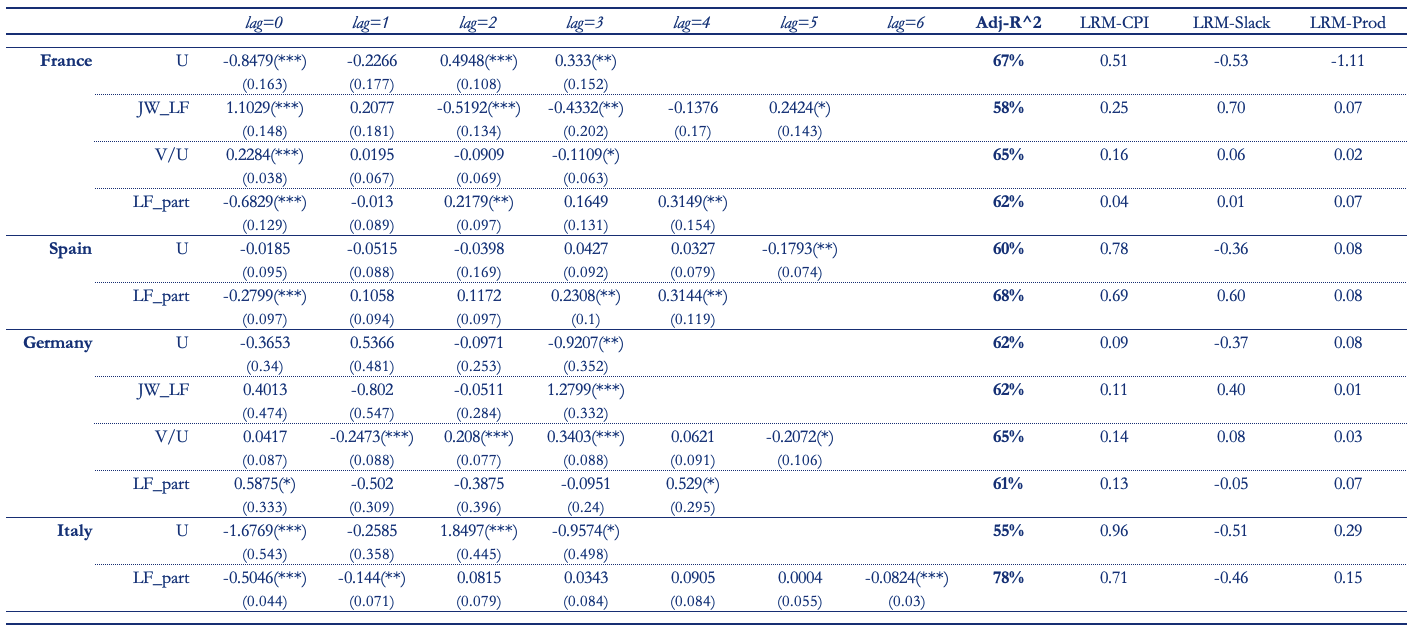
\includegraphics[width=1\textwidth]{Core/2.Labour/img/LRM table.png}
    \label{figure:lrm_table}
\end{figure}
\vspace{-1.5cm}
\noindent \textit{\textbf{NB:} Note that the lack of complete job vacancies series for Italy and Spain forced us to disregard the $V/U$ and $JW\textrm{-}LF$ slack measures for these countries.}

\quad The first thing to note is that no model is completely left-out performance-wise, as almost all show adjusted $\textrm{R}^{2}$ above 60\%. 
Considering the unemployment rate estimate as the baseline the results show that for Germany the job-worker gap and labour force participation measure up to it. 
We estimate that the vacancy-to-unemployment ratio even has a slight edge over other slack measures, with its adjusted $\textrm{R}^{2}$ reaching 65\%. 
Moreover, there does not seem to be a discrepancy in the estimated long-run effect of either CPI or labour productivity. 
We estimate that a permanent increase of 10bps in the QoQ difference of the unemployment rate would lead to a decrease of around 3.7bps in QoQ wage growth. 
The estimated long-run multiplier is close to zero and slightly negative for growth in labour force participation. 
Looking at the data the latter has kept increasing steadily over the past 30 years, almost following a linear trend, from 76\% to as high as 91\%. 
This unstoppable-like upward trend, combined with rising labour force participation even during crises, could explain the estimation of no long-term effect on wage growth. 
Moreover, the threefold combination of effects from changes in unemployment, employment and population might blur the link with wage growth changes. 
See for example Figure \ref{figure:lfpart} for the different drivers in the recent changes in the labour force participation rate, compared to Q4 2019, among our 4-country dataset. 
Finally, both the vacancies to unemployment ratio and the job worker gap show expected positive signs for the LRM estimate. 

\begin{figure}[H]
    \centering
    \caption{Labour force participation breakdown, 2022Q4 against 2019Q4}
    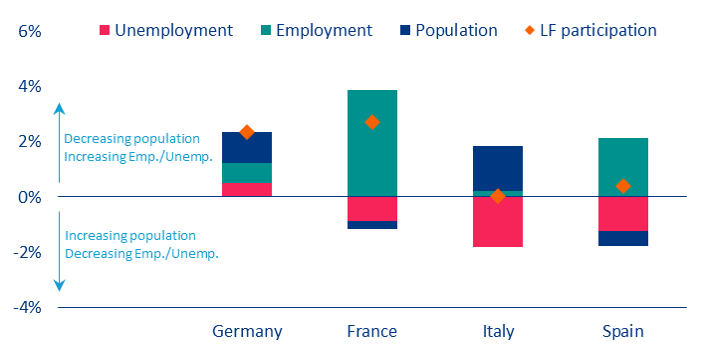
\includegraphics[width=.7\textwidth]{Core/2.Labour/img/lfpart breakdown.png}
    \label{figure:lfpart}
\end{figure}

Regarding France, the models with unemployment, $V/U$ and labour force participation are the best performing with adjusted $\textrm{R}^{2}$ between 62\% and 67\%, though no additional slack measure seems to outperform the model using the first. 
The strong negative estimate for the long-run multiplier of productivity is surprising. 
Compared to an estimation with a sample lasting until Q3 2019, it seems the pool of estimated models deeply embedded the trend rupture in productivity since the break that happened during the Covid crisis and the recent decoupling between wage developments and productivity changes. 
Other slack measures also point to a really low long-run effect (positive but close to zero). 
Similarly to its German counterpart, a decrease of around 5.3bps in QoQ wage growth is estimated from a permanent increase of 10bps in the QoQ difference of the unemployment rate. 
Again, the JW-LF and the V/U ratio both show expected positive signs and estimates are within the same range as for Germany. 
The job-worker gap seems to impact more the French economy than its German counterpart while it is the other way around for the $V/U$ ratio, which probably reflects structural differences between the two countries’ labour market. 

Regarding Spain and Italy, both show improvements when using labour force participation in terms of adjusted $\textrm{R}^{2}$. 
However, compared to France and Germany, the amplitude of estimated long-run effects is on a totally different scale, especially for Italy where it is surprisingly negative. 
For Spain, the estimate is large and positive. 
We guess that for the Italian labour force participation, as it has remained in the same range across the sample, the model overshoots its recurrent slow negative trends during crises and the break during Covid only amplified that. 
As for Spain, the early 2000s’ increase could be overestimated and this past trend would be over-embedded within the model. 

Overall, the different models suggest (again through the long-run multiplier) that -on average- higher inflationary pressures affect the peripheral countries -i.e. Italy and Spain – than the core countries – i.e. France and Germany. 
For the latter, a 1\% increase in QoQ\% inflation would lead to respectively a 12bps increase in wage growth in Germany, and twice as big in France at 24bps. 
In peripheral countries, it reaches 74bps in Spain and up to 84bps in Italy. 
Roberta’s take is that this probably reflects the influence of unions in wage bargaining in peripheral countries, where negotiations take time and gradual wage increases (lower than current inflation) are often preferred in exchange for job security, particularly the case for Spain in 2022. 
However, this also suggests that the contribution of inflation to wage growth in 2023-24 is likely to be more pronounced in Spain and Italy than in the core countries -even though headline inflation has slowed down- as lagged inflationary effects kick in.

We find that labour productivity is the hardest variable whose long-run effect we have to interpret, as a more structural variable and not as easy to grasp as inflation or unemployment. 
We note that there is again a discrepancy between the peripheral and core countries. 
Both Germany and France show a weak to even negative long-term trend in labour productivity effect on wage growth while for Spain and Italy, the estimates are larger and positive. 
Compared to France it seems the recent dip in Spanish labour productivity has not (yet) changed the positive relationship between productivity and wage growth, despite the two countries showing similar breaks and no recovery, probably because for France the decrease in productivity was stronger despite strongly rising labour cost.

Then, to select the ‘best’ model for our analysis, we not only rely on the adjusted $\textrm{R}^{2}$ value but also on the availability of forecasts for the different series. 
As we do not have forecasts of vacancies, despite the marginal gains in explaining wage developments, we had to drop the $V/U$ and $JW\textrm{-}LF$ models if we were to use them to compute forecasts. 
With the unemployment rate being a key variable in the team’s labour market outlook, each economist has to produce quarterly forecasts which are then debated and confirmed for the scenario. 
The general interest in a forecasting model using this specific variable, the confidence in the forecasted series and the overall results’ performance motivated the selection of the estimated models using the unemployment rate.

\subsection{Wage growth models results}

\quad The table below displays the full estimates for each country. 
Charts plotting the selected model estimate and the top 25\% of $\textrm{R}^{2}$-models against actual values can be found in the annexe (Figure \ref{figure:fr25} to \ref{figure:it25}).

\begin{figure}[H]
    \centering
    \caption{Best model selected for each slack variable}
    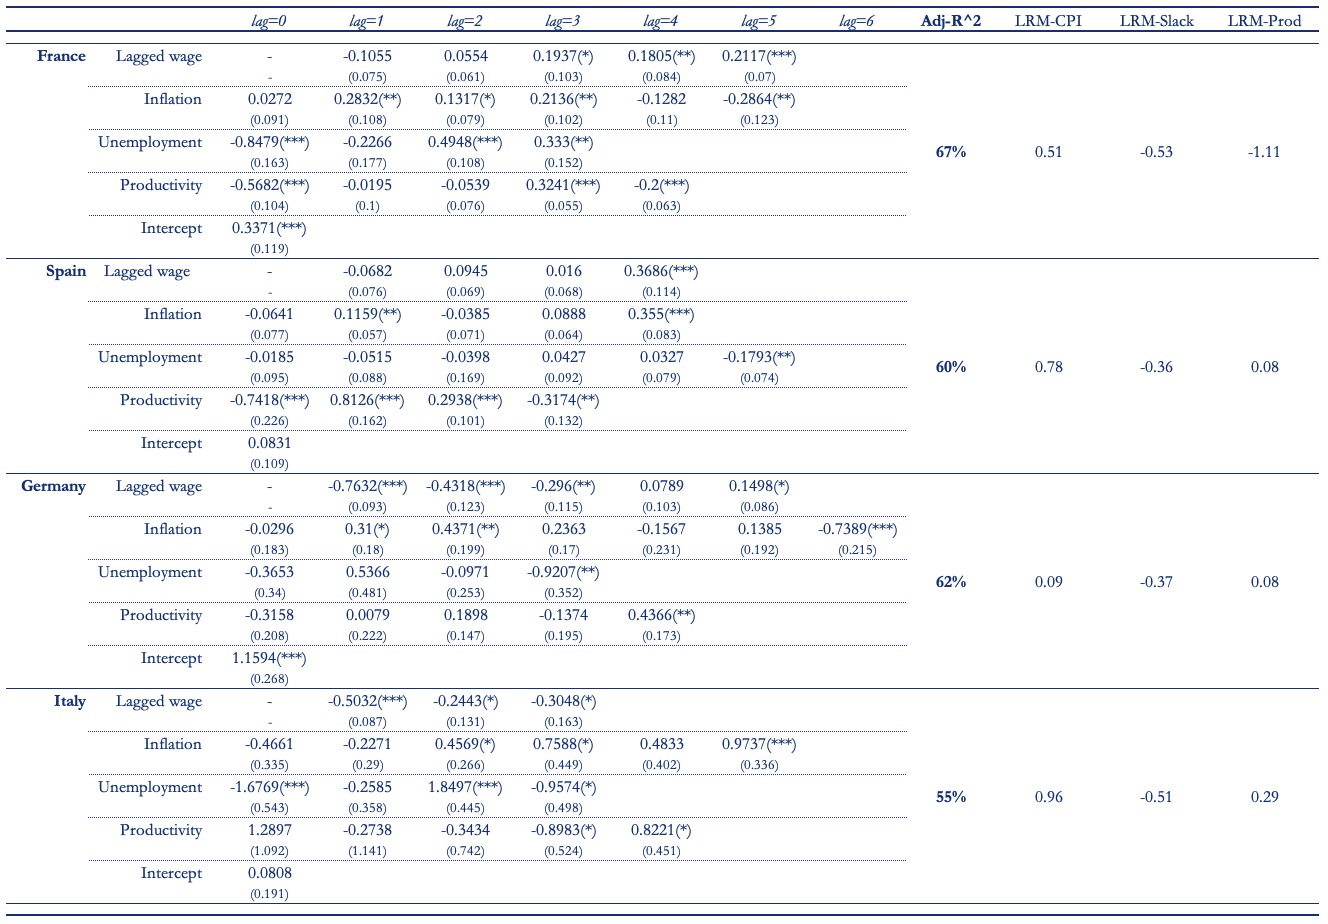
\includegraphics[width=.87\textwidth]{Core/2.Labour/img/labour_results.png}
    \label{figure:labour_results}
\end{figure}
\vspace{-1cm}
As we have mostly gone over the parameters’ interpretation before, we focus on decomposing wage growth using these models (Beta-variation figures \ref{figure:frbreakdown} to \ref{figure:itbreakdown}) and assess both recent drivers and expectations for 2023 and the first semester of 2024. 
Note that as we worked on this project around March/April 2023, for a publication and the Q2 scenario around the same date, the first two quarters of the year are included in the forecast timeframe. 
We first look at the results for the core countries.

\begin{figure}[H]
    \centering
    \caption{Model-based wage growth breakdown for France \& average contribution by component.}
    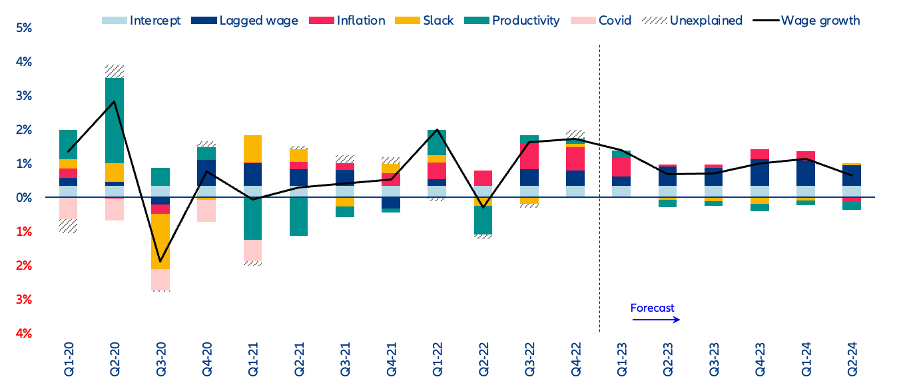
\includegraphics[width=.8\textwidth]{Core/2.Labour/img/Franceb1.png}
    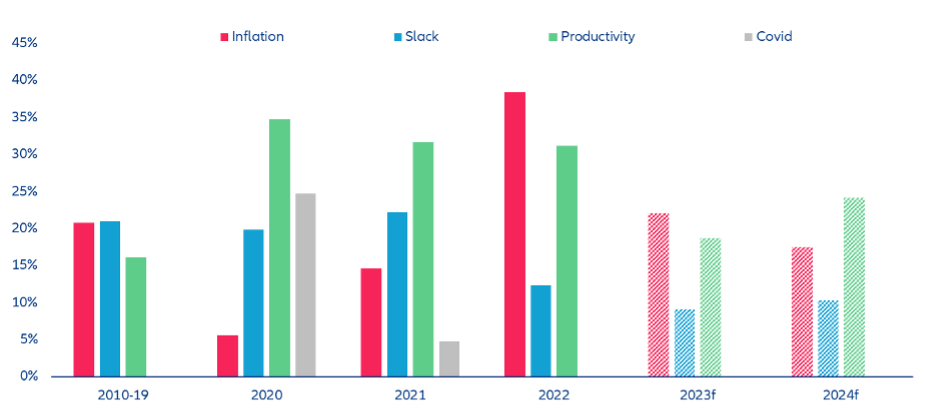
\includegraphics[width=.8\textwidth]{Core/2.Labour/img/Franceb2.png}
    \label{figure:frbreakdown}
\end{figure}

Regarding the French economy, the model suggests the pandemic affected wage growth mainly through changes in labour productivity and the unemployment rate. 
The Covid dummy variable coefficient estimate, which aims at estimating on average the temporary pandemic disruption not coming from the included variables, is negative (-0.64) and significant at the 5\% level. 
We note the chosen model performs particularly well during the pandemic period. 
It appears labour productivity has been a statistically key variable over the past two years, with large changes. 
In our view, the model shows to some extent some balancing effects in labour productivity, as the largest coefficient estimates are for the contemporaneous value and the lag 3 with opposite signs (negative then positive). 
We believe the strong negative coefficient for the lag 0 comes from the opposite contemporaneous changes in wage growth and labour productivity observed in the data while other lags, and especially the third, could reflect the positive link with the trend of productivity growth rather than precisely one-for-one immediate changes (the topic is also addressed in these two papers: Dew-Becker and Gordon 2005; Yellen 2005). 
Over the past three years, changes in labour productivity have accounted for, on average, around 33\% of wage growth. 
We expect this contribution to decrease to 22\% in 2023-24, returning close to its pre-pandemic average (17\%). 
The falling labour productivity trend suggests downward pressures on wage growth, visible with negative contributions from Q2 2023 onwards. 

In the same vein, weaker growth economic prospects point to a relative increase in the unemployment rate (remaining close to its lower historical bound) limiting once again prospects of increases in wages. 
The pandemic being a pretty peculiar period, our main focus for inflation is recent developments, especially since late 2021. 
The figure shows that rising inflationary pressures on wages started as early as Q4 2021 before quickly rising in Q3 and Q4 2022, following the Russian invasion of Ukraine in March 2022 and the economic turmoil it engendered. 
It is consistent with the worldwide increase in inflation that started around mid-2021, attributed in part to supply chain problems and supply shortages amid recovery in consumer demand. 
The country also suffered from higher imported prices, due to already rising energy prices. 
With inflation’s contribution to QoQ wage growth rising as high as 45\% and 50\% in Q2 and Q3 2022, the model suggests that after Q1 2023 at the same level, inflationary pressures on wages are to significantly decrease but remain positive. 
Thus, this suggests there should not be disinflation passing through to wages and we could expect positive real wage growth. 
Overall, according to model-based forecasts, we should expect an average yearly wage growth of 4.7\% in 2023 and 2.7\% in 2024 (keep in mind that our measure of wage uses the logarithm of the Hourly earn, hence another reason that our figures may differ from central bank’s estimates…).

\begin{figure}[H]
    \centering
    \caption{Model-based wage growth breakdown for Germany \& average contribution by component.}
    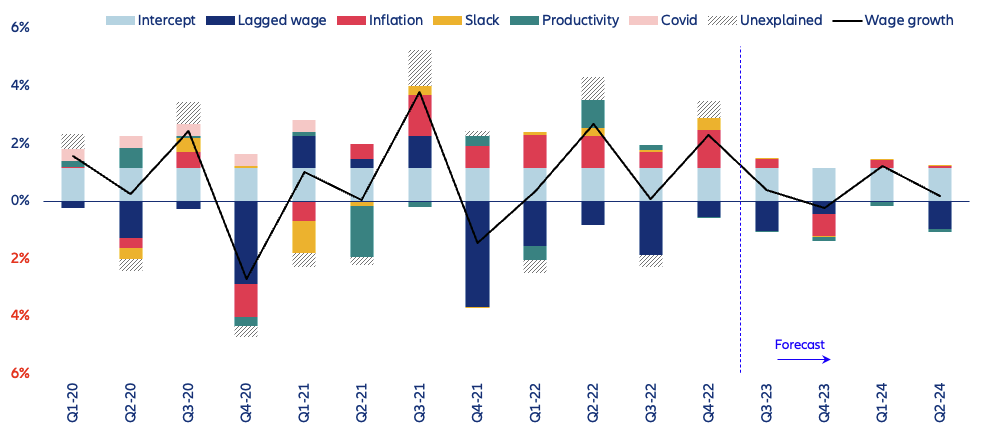
\includegraphics[width=.8\textwidth]{Core/2.Labour/img/germanyb1.png}
    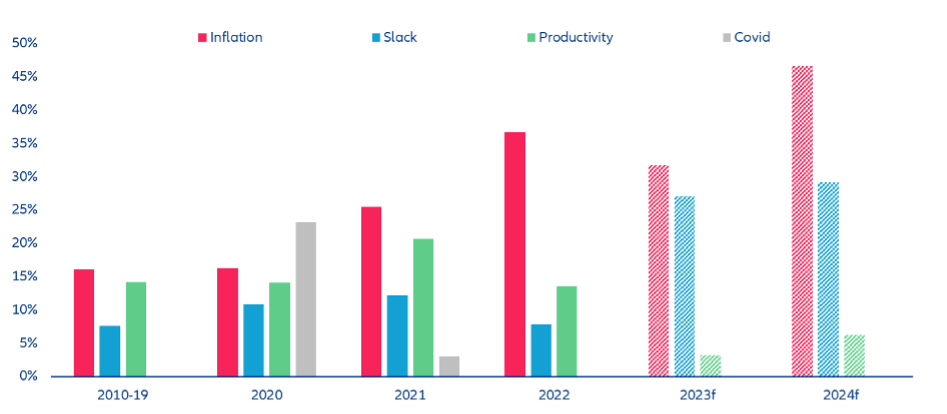
\includegraphics[width=.8\textwidth]{Core/2.Labour/img/germanyb2.png}
    \label{figure:gerbreakdown}
\end{figure}

It appears that, during the pandemic, wage growth in Germany was not as heavily influenced by labour productivity changes as its French counterpart. 
However, inflationary pressures arose sooner and stronger. 
The surge in inflation from mid-2021 onwards accounts for 50\% of the QoQ growth rate in Q3 2021 and on average 30\% between Q4 2021 and Q2 2022. 
The model suggests the pass-through of the war in Ukraine-induced inflation (energy-induced inflation) should be more limited in Germany compared to France, with a moderate contribution (20\%) in Q3 2022 and a peak in the following quarter (60\%). 
On the other hand, the inflation pathway used in the forecast also points to possible deflationary effects in late 2023. 
Again, without strong unexpected changes in the unemployment rate, we do not expect it to be that strong of a driver for wage growth. 
The figure also shows a higher estimate for Germany than for France, which can somewhat be interpreted as the structural level around which QoQ wage growth fluctuates. 
Overall, the model-based estimates still appear to fall short compared to the 4.5\% estimate by the Deutsche Bundesbank, with yearly wage growth estimates of 3.3\% in 2023 and 2.2\% in 2024. 
This probably reflects differences in inflation pathways, as the German bank may embed core inflation -which they expect to remain high- into their model rather than headline inflation. 
There are also expected inflation adjustment premiums instruments, one-off payments “inflation compensation bonuses”, which will boost effective earnings. 

\begin{figure}[H]
    \centering
    \caption{Model-based wage growth breakdown for Spain \& average contribution by component.}
    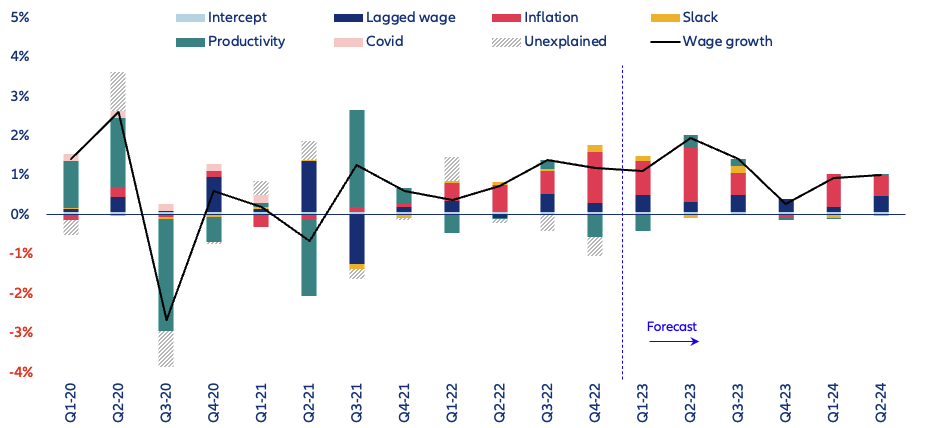
\includegraphics[width=.8\textwidth]{Core/2.Labour/img/spainb1.png}
    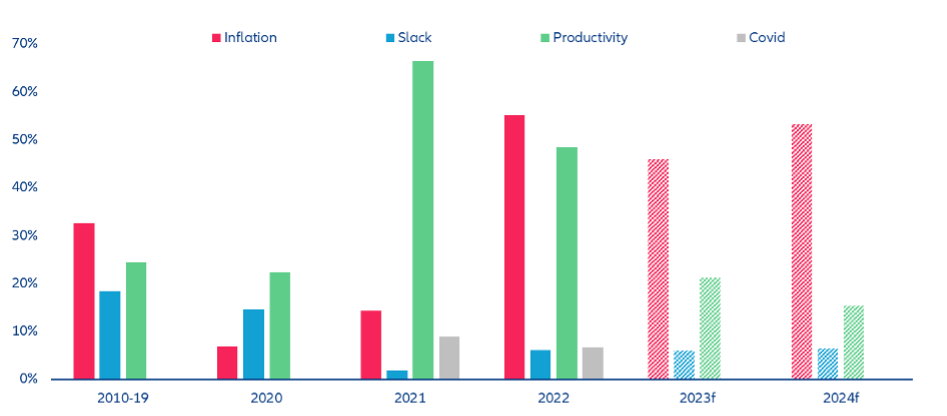
\includegraphics[width=.8\textwidth]{Core/2.Labour/img/spainb2.png}
    \label{figure:spbreakdown}
\end{figure}

Similarly to France, the Spanish model suggests labour productivity changes during the pandemic drove most of the changes in wage growth. 
However, the QoQ difference in the unemployment rate doesn’t appear to matter as much in comparison. 
Our pathway projects some little increases in the unemployment rate between Q3 2023 and Q1 2024, but overall it should not be a strong driver of future wage growth. 
We also note the model shows some struggle during the early stages of the pandemic (Q2-Q3 2020). 
What is more striking is the increasing pressures of inflation on wages, not really in 2021, but from Q1 2022 and onwards. 
In 2022, the contribution of inflation to QoQ wage growth increased from 45bps in Q1 to 130bps in Q4. 
This is well above what we have seen for the core countries but more importantly, the surge appears delayed in comparison. 
Looking at the coefficient estimates for the different lags of the inflation variable, the latest one included (lag 4) is positive, significant at 1\% and dominates the other lags ($\beta = 0.36$ compared to -0.06, 0.12, -0.04 and 0.09). 

What it tells us is that the previous year's (QoQ) inflation rate will mainly determine the inflation component of the current wage growth, and thus the with current level of inflation we can have a first intuition regarding wage growth for the year ahead. 
As we have already mentioned, this probably reflects lengthy and gradual wage negotiations that happen over time but it also indicates that the quarterly increases in inflation we have seen between Q2 and Q4 2022 (namely 2\%, 3\% and 1\%) have not yet fully passed through to wages. 
If headline inflation is to moderate on the back of lower energy prices, the Spanish Central Bank could potentially face the challenge of rapid wage adjustment kicking in as soon as Q2 2023 -with the model suggesting a peak in QoQ wage growth at 2\%- which, in addition to the 8\% increase in the minimum wage (government and unions agreed on a deal in early February), could feed into higher core inflation. 
Overall, inflation contribution amounts to 55\% in 2022 and we expect it to remain around 50\% in the upcoming two years due to high past inflation. 
Without drastic changes in employment or GDP, we also expect the contribution of labour productivity to continue decreasing and to revert to pre-pandemic levels in 2023. 
Our model-based wage growth forecast for 2023 and 2024 project year-on-year increases of 4.7\% and 4.2\%.

\begin{figure}[H]
    \centering
    \caption{Model-based wage growth breakdown for Italy \& average contribution by component.}
    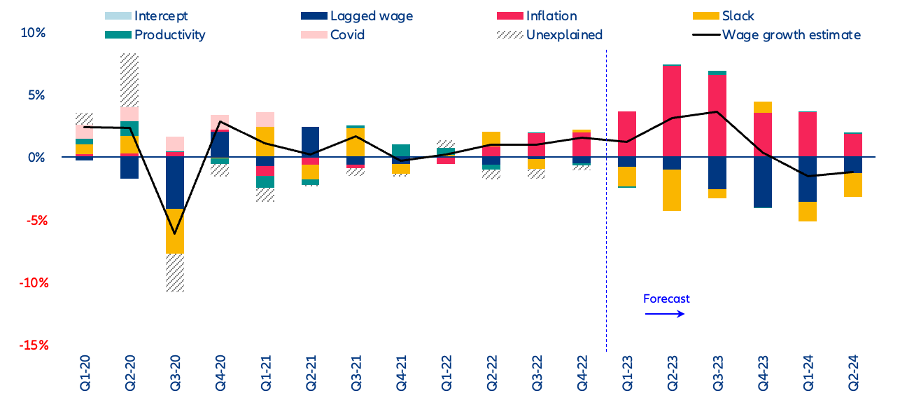
\includegraphics[width=.8\textwidth]{Core/2.Labour/img/italyb1.png}
    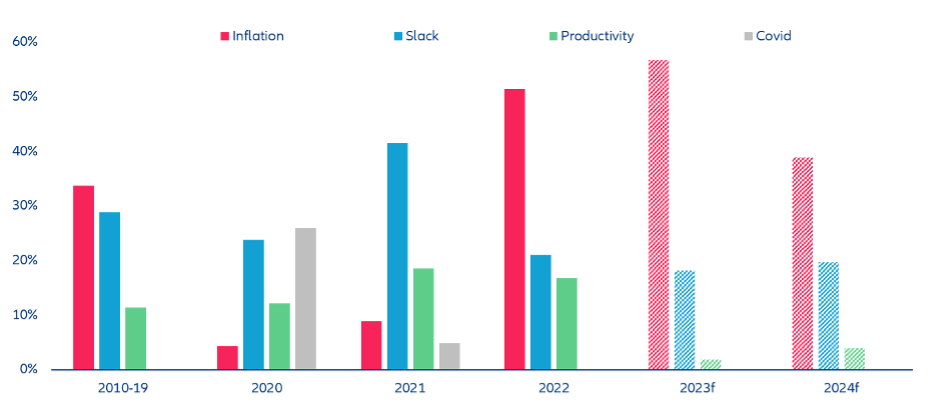
\includegraphics[width=.8\textwidth]{Core/2.Labour/img/italyb2.png}
    \label{figure:itbreakdown}
\end{figure}
\newpage

Compared to the other three countries of our study quarterly changes in the unemployment rate are much more influencing wage growth in Italy. 
The average contribution of slack to wage developments amounts to around 30\% for the 2010 to 2019 period. 
During the pandemic, it rose from 25\% in 2020 to as high as 45\% in 2021, while changes in labour productivity appear not to have affected wage growth as much as in Spain or France to some extent. 
In addition, our pathway expects very little changes in labour productivity, thus the low contribution. 
We note that Italy has the chosen model that shows the most struggle to explain wage growth at the offset of the Covid-19 crisis, the dummy variable is not enough to model a surge in Q2 2020 than a strong drop in Q3 of the same year. 
In hindsight, it could have been better to use two separate dummy variables for that purpose. 
Our forecast pathway projects the unemployment rate to increase from Q4 2022 onwards, going up from 7.8\% to 8.45\% by early 2024, putting downward pressure on wages. 
After returning to pre-pandemic levels in 2022 the overall contribution of slack should remain around 20\% for 2023-2024. 

Similarly to the Spanish case, inflationary pressures appear delayed around Q2-Q3 2022 and in the last semester of that year the model suggests it explains over 65\% of wage growth. 
Looking at the breakdown details, it appears the contribution of inflation for the last semester of 2022 is mainly driven by inflation from the past 2 to 5 quarters. 
This is particularly relevant when assessing future wage growth for Italy as the country has recorded extremely high QoQ inflation rates throughout 2022, between 1.8\% in Q2 to as high as 4.2\% in Q4. 
The model then projects a strong pass-through of inflation to QoQ wage growth in 2023, contributing to around 60\% of the whole year's changes in wages. 
The model-based forecast project wage growth at 6.7\% for 2023 and 3.5\% for 2024.

\subsection{Changes in labour productivity}

\quad Labour productivity (which we defined as GDP over Employment) is a key topic when assessing the state of an economy and its outlook, as it is a driver of economic growth and it affects all players in the economy (businesses, workers and the government) through different channels whether it is output (same output with less -human resources- hours worked/workers), likely higher wages or higher tax revenues. 
To understand its contribution to the wage growth breakdowns above we also worked on a breakdown on its own for productivity using the number of hours worked per employee and the output produced per hour (\ref{prod1}). 
The GDP per hour is also decomposed to assess the possible effect of Employment (\ref{prod2}). We compare Q4 2022 labour productivity to pre-Covid level (Q4 2019). 
The two charts below and the country-specific and quarterly breakdown allow us to highlight the following points.

\begin{align}
    \frac{GDP}{E} &= \frac{GDP}{Hours}.\frac{Hours}{E} \longmapsto \textrm{\textit{Productivity}}\% \sim \frac{GDP}{Hours}\% - \frac{Hours}{E}\% \label{prod1}\\
    \nonumber \\
    \frac{GDP}{Hours} &= \frac{GDP}{\frac{Hours}{E}.E} \longmapsto \textrm{\textit{GDP/Hour}}\% \sim GDP\% - ( \frac{Hours}{E}\% + E\%) \label{prod2}
\end{align}

\begin{figure}[H]
    \centering
    \caption{Latest Labour productivity breakdown (Q4 2022 vs Q4 2019).}
    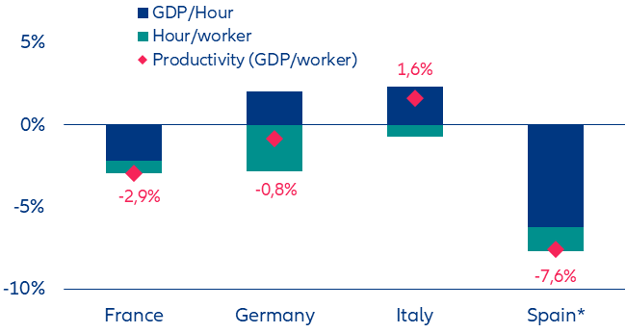
\includegraphics[width=.6\textwidth]{Core/2.Labour/img/prodbreakdown1.png}
    \label{figure:prodbreakdown1}
\end{figure}
\vspace{-.5cm}
\quad \quad \quad \textit{\textbf{NB:} $\textrm{Spain}^{*}$ breakdown for Q3 2022}
\begin{figure}[H]
    \centering
    \caption{Latest GDP/Hour breakdown (Q4 2022 vs Q4 2019).}
    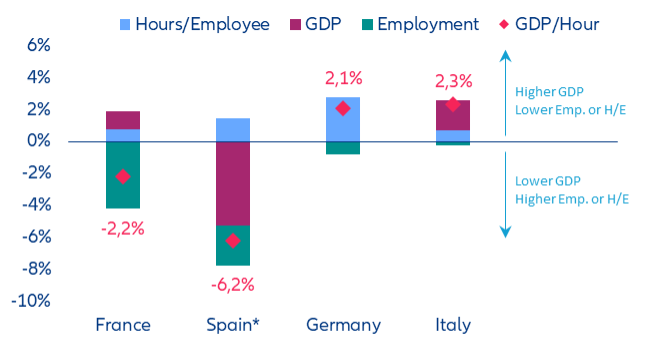
\includegraphics[width=.6\textwidth]{Core/2.Labour/img/prodbreakdown2.png}
    \label{figure:prodbreakdown2}
\end{figure}
\vspace{-.5cm}
\quad \quad \quad \textit{\textbf{NB:} $\textrm{Spain}^{*}$ breakdown for Q3 2022}

Out of the four countries we considered only Italy shows remarkable growth in productivity compared to Q4 2019, with the other European economies lagging. 
Productivity growth is still in the red in France and especially in Spain relative to pre-pandemic levels while the decline has been relatively small in Germany. 
For the latter, the decline in Hours worked per worker has been compensated by a pick-up in GDP per Hour. 
Employment has slightly increased compared to Q4 2019 and GDP recovered to pre-pandemic levels (from the -10\% drop in Q2 2020, it went back to 2019 levels in early 2022), the change in GDP/Hour is thus mostly driven by the decrease in Hours worked per Employee. 
Thus, the overall effect on labour productivity is only a matter of Employment, which slightly improved at constant GDP and explains the -0.8\%.

In France, the situation is pretty different as the country shows a larger loss in labour productivity (-2.9\%). 
What is striking is the strong increase in employment compared to Q4 2019, which reduces the need to increase efficiency and productivity. 
We have seen a rapid acceleration in job creation since 2021, especially regarding youth employment and apprentices. 
The employment rate for 15-24 years old has increased by +4.6pps between end-2019 and end-2022, against +2.0pps for the 25-49 age group and +3.1pps for the 50-64 cohort. 
The increase in GDP from the pre-pandemic level still does not fully compensate for the strong employment effect (the country recovered from the Q2 2020 -17\% drop in Q3 2021).

Spain being the top productivity underperformer can be attributed to, on the one hand, a strong decline in GDP and on the other hand a strong increase in employment. 
Looking at the quarterly breakdown, Spanish GDP has not yet fully recovered from Q2 2020 GDP being down 21\% compared to Q4 2019 as it remains in Q3 2022 at around -5\%. 
Regarding employment, it started increasing as early as Q4 2021 and stands at +3\% in Q3 2023. 
Spain has seen strong employment growth among the younger cohorts but also among the older cohort – +6.5\% and +10.3\%, respectively. 
At the same time, employment growth for the 24-49 age group declined.

Lastly, Italy has been the only country showing gains in labour productivity from 2020 onwards. 
Similarly to other European countries, the country’s labour market has adjusted to the Covid-19 crisis via reduced working hours rather than layoffs. 
But at the same time, the Italian labour market differs from the other three as the countries have witnessed unemployment levels well above the one in Q4 2019 (thus decreases in employment) throughout 2020 and mid-2021. 
During this year and a half, employment has been between 7\% and 20\% below the levels seen in late 2019. 
Over the same period, GDP shrank (-15\% in Q2 2020) but recovered from Q4 2021 onwards. 
The decline in working hours per employee was thus more than compensated by increasing GDP/Hour as the positive effect of the decrease in employment was, until Q3 2021, always higher than the negative effect of GDP. 
From Q4 2021 onwards, both positively contributed to changes in GDP/Hour which led overall to positive changes in labour productivity, standing at +1.8\% as of Q3 2022. 

\subsection{Summary of key findings}
\begin{itemize}
    \item We find that other measures of slack can perform as best as (and sometimes better) the unemployment rate to explain wage growth. The different measures also all point towards discrepancies in inflationary pressures on wages in the peripheral countries than in the core countries.
    \item Wage growth has been strengthening over the past year, supported by robust labour markets and some catch-up in wages to compensate workers for high inflation. While this is likely to decelerate as inflation eases and the economy slows further in core countries, peripheral countries could potentially be challenged with delayed rapid wage increases which could put further pressure on core inflation.
    \item There has been divergent dynamics within the Eurozone regarding productivity changes due to structural factors, underscoring the need for a nuanced approach in addressing productivity disparities among member states.
\end{itemize}